
%\documentclass[10pt,proceedings]{IEEEtran}
%\documentclass[a4paper, 10pt, conference]{ieeeconf}      % Use this line for a4 paper

\documentclass[letterpaper, 10 pt, proceedings]{ieeetran}  % Comment this line out
%\IEEEoverridecommandlockouts                              % This command is only


\usepackage{geometry}
\usepackage{graphicx}
\graphicspath{{./Figures/}}
\usepackage{amsmath}
%\usepackage{amsfonts}
\usepackage{amsthm}
%\usepackage{stfloats}
\usepackage{caption}
\usepackage{float}
\usepackage{mathrsfs}
\usepackage{placeins}
\usepackage{subcaption}
\geometry{letterpaper,top=.75in,left=.69in,bottom=.75in,right=.69in}
\pagestyle{empty}


\newcommand{\A}{_{\textsc{\tiny \textit{A}}}}
\newcommand{\B}{_{\textsc{\tiny \textit{B}}}}
\newcommand{\D}{_{\textsc{\tiny \textit{D}}}}
\newcommand{\T}{_{\textsc{\tiny \textit{T}}}}
\newcommand{\G}{_{\textsc{\tiny \textit{G}}}}
\newcommand{\R}{_{\textsc{\tiny \textit{R}}}}
\newcommand{\sub}[1]{_\textsc{\tiny \textit{#1}}}
\newcommand{\sgn}{\text{sgn}}

\newtheorem{thm}{Theorem}


\title{\LARGE \bf
	Report 2: Examining the impact of risk preference and networked based decision making on brokers in the stock market
}

\author{Rachael Judy, Connor Klein, Josh Smith% <-this % stops a space
}


\begin{document}
	
	\maketitle
	\thispagestyle{empty}
	\pagestyle{empty}
	
	%	\begin{abstract}
		%		Using some of the theories from Taleb regarding antifragility, construct a network of firms and networked brokers inside firms to explore the impact of different preferences for risk as well as impact of weighting neighbors actions in decisions. 
		%	\end{abstract}
	
	\section{Current Status}
	
	\begin{figure}
		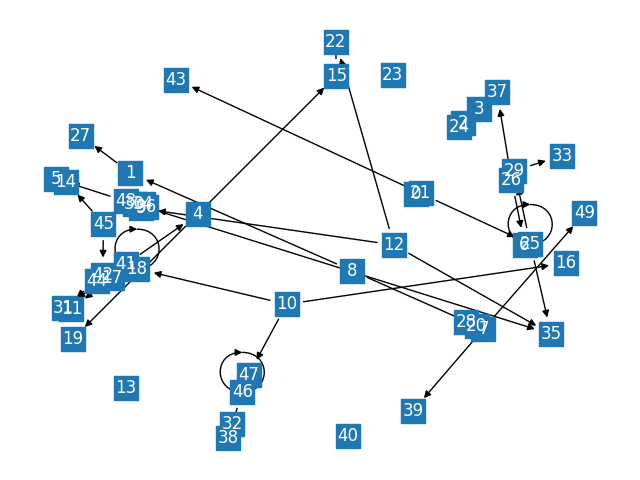
\includegraphics[width=.5\textwidth]{samplegraph.png}
		\caption{Sample graph generated}
		\label{samplegraph}
	\end{figure}
	
	
	
	%
	
	\bibliographystyle{ieeetran}
	\begin{thebibliography}{99}	
		\bibitem{antifragile}
		N. N. Taleb, Antifragile: Things that gain from disorder. Harlow, England: Penguin Books, 2013.
		
		\bibitem{networkscrowdsmmarkets}
		D. Easley and J. Kleinberg, Networks, crowds, and markets: Reasoning about a highly connected world. Cambridge, England: Cambridge University Press, 2012.
		%- https://www.cs.cornell.edu/home/kleinber/networks-book/, particularly chapters 9-12, 17, 22
		
		\bibitem{neuralnets}
		A. Thakkar and K. Chaudhari, “A comprehensive survey on deep neural networks for stock market: The need, challenges, and future directions,” Expert Systems with Applications, vol. 177, p. 114800, Sep. 2021, doi: 10.1016/j.eswa.2021.114800.
		%- https://www.sciencedirect.com/science/article/pii/S0957417421002414
		
		\bibitem{complexmacroeconomics}
		C. Hommes, “Behavioral and Experimental Macroeconomics and Policy Analysis: A Complex Systems Approach,” Journal of Economic Literature, vol. 59, no. 1, pp. 149–219, Mar. 2021, doi: 10.1257/jel.20191434.
		%- https://pubs.aeaweb.org/doi/pdfplus/10.1257/jel.20191434
		
		\bibitem{networkstocks}
		C. K. Tse, J. Liu, and F. C. M. Lau, “A network perspective of the stock market,” Journal of Empirical Finance, vol. 17, no. 4, pp. 659–667, Sep. 2010, doi: 10.1016/j.jempfin.2010.04.008.
		%- https://www.sciencedirect.com/science/article/pii/S0927539810000368
		
		\bibitem{marketcrasheswikipedia}
		“List of stock market crashes and bear markets,” Wikipedia. Jan. 24, 2024. Accessed: Feb. 13, 2024. [Online].
		%- dates noted as stock crashes (https://en.wikipedia.org/wiki/List_of_stock_market_crashes_and_bear_markets)
		
		\bibitem{antifragile}
		N. N. Taleb, Antifragile: Things that gain from disorder. Harlow, England: Penguin Books, 2013.
		
		\bibitem{networkscrowdsmmarkets}
		D. Easley and J. Kleinberg, Networks, crowds, and markets: Reasoning about a highly connected world. Cambridge, England: Cambridge University Press, 2012.
		%- https://www.cs.cornell.edu/home/kleinber/networks-book/, particularly chapters 9-12, 17, 22
		
		\bibitem{neuralnets}
		A. Thakkar and K. Chaudhari, “A comprehensive survey on deep neural networks for stock market: The need, challenges, and future directions,” Expert Systems with Applications, vol. 177, p. 114800, Sep. 2021, doi: 10.1016/j.eswa.2021.114800.
		%- https://www.sciencedirect.com/science/article/pii/S0957417421002414
		
		\bibitem{complexmacroeconomics}
		C. Hommes, “Behavioral and Experimental Macroeconomics and Policy Analysis: A Complex Systems Approach,” Journal of Economic Literature, vol. 59, no. 1, pp. 149–219, Mar. 2021, doi: 10.1257/jel.20191434.
		%- https://pubs.aeaweb.org/doi/pdfplus/10.1257/jel.20191434
		
		\bibitem{networkstocks}
		C. K. Tse, J. Liu, and F. C. M. Lau, “A network perspective of the stock market,” Journal of Empirical Finance, vol. 17, no. 4, pp. 659–667, Sep. 2010, doi: 10.1016/j.jempfin.2010.04.008.
		%- https://www.sciencedirect.com/science/article/pii/S0927539810000368
		
		\bibitem{marketcrasheswikipedia}
		“List of stock market crashes and bear markets,” Wikipedia. Jan. 24, 2024. Accessed: Feb. 13, 2024. [Online].
		
		\bibitem{kulmann}
		M. Kuhlmann, "Explaining financial markets in terms of complex systems," \textit{Philosphy of Science}, vol. 81, no. 5, pp. 1117-1130, Dec. 2014. %doi: 10.1086/677699.
		
		\bibitem{dimaggio_relevancebrokernetworks}
		M. Di Maggio, F. Franzoni, A. Kermani, and C. Sommavilla, "The relevance of broker networks for information diffusion in the stock market," \textit{Journal of Financial Economics}, vol. 134, no. 2, pp. 419-446, Nov. 2019. %doi: 10.1016/j.jfineco.2019.04.002. 
		
		
		\bibitem{gai_contagion}
		P. Gai and S. Kapadia, "Contagion in financial networks," \textit{Proceedings of the Royal Society}, vol. 466, no. 2120, pp. 2401–2423, Aug. 2010.
		
		\bibitem{liu_networkperspective}
		C. K. Tse, J. Liu, and F. C. M. Lau, “A network perspective of the stock market,” \textit{Journal of Empirical Finance}, vol. 17, no. 4, pp. 659–667, Sep. 2010. % doi: 10.1016/j.jempfin.2010.04.008.
		
		\bibitem{li_correlation}
		G. Li, A. Zhang, Q. Zhang, D. Wu, and C. Zhan, “Pearson correlation coefficient-based performance enhancement of broad learning system for stock price prediction,” \textit{IEEE Transactions on Circuits and Systems II: Express Briefs}, vol. 69, no. 5, pp. 2413–2417, May 2022. %, doi: 10.1109/TCSII.2022.3160266.
		
		\bibitem{fiedor_networksmutualinformationrate}
		P. Fiedor, “Networks in financial markets based on the mutual information rate,” \textit{Physical Review E}, vol. 89, no. 5, May 2014. % doi: 10.1103/PhysRevE.89.052801.
		
		\bibitem{cooper_realinvestmentandrisk}
		I. Cooper and R. Priestley. "Real investment and risk dynamics," \textit{Journal of Financial Economics}, vol. 101, no. 1, pp. 182-205, July 2011.
		
		\bibitem{lansing_riskaversion}
		K. J. Lansing and S. F. LeRoy, “Risk aversion, investor information and stock market volatility,” \textit{European Economic Review}, vol. 70, pp. 88-107, July 2014. 
		
		\bibitem{risktolerance}
		J. E. Corter and Y. J. Chen, “Do investment risk tolerance attitudes predict portfolio risk?,” \textit{Journal of Business and Psychology}, vol. 20, no. 3, pp. 369-381, 2006.
		
		\bibitem{harmon_economicinterdependence}
		D. Harmon, B. Stacey, Y. Bar-Yam, and Y. Bar-Yam, "Networks of economic market interdependence and systemic risk," New England Complex Systems Institute, Cambridge, MA, Tech. Report 1011.3707, Mar. 2009.
		
		\bibitem{park_complex}
		J. Park, C. H. Cho, and J. W. Lee, "A perspective on complex networks in the stock market," \textit{Frontiers in Physics}, vol. 10, Dec. 2022. %[Online serial] %, doi: 10.3389/fphy.2022.1097489.
		
		\bibitem{baydelli_hierarchicalmarket}
		Y. Y. Baydilli, S. Bayir, and I. Tuker, “A hierarchical view of a national stock market as a complex network,” \textit{Economic Computation \& Economic Cybernetics Studies \& Research}, vol. 51, no. 1, pp. 205–222, Jan. 2017.
		
		
	\end{thebibliography}
	
	
\end{document}
